\documentclass{article}
\usepackage[utf8]{inputenc}
\usepackage{enumitem}
\usepackage{titling} % Package for customizing the title page
\usepackage{graphicx} % Package for including images
\usepackage{geometry} % Package for adjusting page margins
\usepackage{xcolor} % Package for color customization

% Define colors
\definecolor{titlecolor}{RGB}{0,63,92} % Dark blue
\definecolor{subtitlecolor}{RGB}{0,100,150} % Light blue

% Set page margins
\geometry{margin=2.5cm}

% Redefine \maketitle to include custom title page
\renewcommand{\maketitle}{
    \begin{titlepage}
        \centering
        % Include your project logo
        
\includegraphics[width=0.4\textwidth]{iith_logo.png} 
        \vspace{2cm} % Adjust vertical space
        
        % Title
        {\color{titlecolor}\Huge\bfseries Software Requirements Specification (SRS)\par}
        \vspace{1.5cm} % Adjust vertical space
          {\color{black}\large Group 07\par}
        % Project name
        {\color{subtitlecolor}\Large Project Name: E-commerce Website\par}
        \vspace{0.5cm} % Adjust vertical space
        
        % Group members

        {\fontsize{14}{18}\selectfont Group Members:\par}
        \vspace{0.2cm} % Adjust vertical space
       
{\large
\begin{center}
\begingroup
\setlength{\tabcolsep}{15pt} % change the column separation
\renewcommand{\arraystretch}{2} % change the row separation
\begin{tabular}{|l|l|}
\hline
\textbf{Name} & \textbf{ Roll Number} \\
\hline
K Vivek Kumar & CS21BTECH11026 \\
\hline
Bhende Adarsh Suresh & CS21BTECH11008 \\
\hline
Jarupula Sai Kumar & CS21BTECH11023 \\
\hline
N Sree Harsha & CS21BTECH11042 \\
\hline
\end{tabular}
\endgroup
\end{center}
}


        \vspace{0.5cm} % Adjust vertical space

        % Group number
       
        \vfill
        
        % Date
        {\large\today\par}
        \vspace{1cm} % Adjust vertical space
    \end{titlepage}
}

\title{} % Remove default title
\author{} % Remove default author
\date{} % Remove default date
\begin{document}

\maketitle
\tableofcontents
\newpage
\section{Introduction}
\subsection{Purpose}
The purpose of this document is to outline the requirements for the development of an online platform that facilitates user interaction with products, orders, and profiles. This platform aims to provide a seamless experience for users, administrators, and retailers.

\subsection{Scope}
The scope of this project includes the development of user authentication, profile management, product management, cart functionality, order management, search options, and potential future extensions such as a payment gateway and recommendation system.

\subsection{Overview}
This document will detail the specific requirements for each user type (customer, admin, and retailer), along with functional, performance, design constraints, and external interface requirements.

\section{Overall Description}
\subsection{Product Perspective}
The platform will serve as an intermediary between customers, administrators, and retailers, facilitating interactions related to product browsing, purchasing, and management.

\subsection{Product Functions}
\begin{itemize}[label=-]
    \item User Authentication: Allows users to register, login, and manage their accounts securely.
    \item Profile Management: Enables users to view and edit their profile information.
    \item Product Management: Provides administrators and retailers the ability to add, edit, and delete product listings.
    \item Cart Functionality: Allows users to view cart contents, add items to the cart, and remove items from the cart.
    \item Order Management: Enables users to view order history and generate invoices.
    \item Search Option: Allows users to search for products within the platform.
\end{itemize}

\subsection{User Characteristics}
\subsubsection{Customer Characteristics}
\begin{itemize}[label=-]
    \item Requires authentication for accessing platform features.
    \item Can browse products, add them to the cart, and place orders.
    \item Can view and edit their profile information.
\end{itemize}

\subsubsection{Admin Characteristics}
\begin{itemize}[label=-]
    \item Requires authentication for accessing platform features.
    \item Can manage products, including adding, editing, and deleting listings.
    \item Can view order history and generate invoices.
\end{itemize}

\subsubsection{Retailer Characteristics}
\begin{itemize}[label=-]
    \item Requires authentication for accessing platform features.
    \item Can manage products, including adding, editing, and deleting listings.
    \item Can edit their profile information.
\end{itemize}

\subsection{Principal Actors}
\begin{itemize}[label=-]
    \item Customers: Users who interact with the platform to browse and purchase products.
    \item Admins: Users responsible for managing the platform, including product listings and orders.
    \item Retailers: Users who list their products on the platform for sale.
\end{itemize}

\subsection{General Constraints}
\begin{itemize}[label=-]
    \item The platform must ensure secure user authentication and data management.
    \item Performance must meet acceptable standards for response times and system reliability.
\end{itemize}

\subsection{Assumptions and Dependencies}
\begin{itemize}[label=-]
    \item The platform will be developed using appropriate technologies and frameworks.
    \item Integration with external services such as payment gateways may be required for future extensions.
\end{itemize}

\section{Specific Requirements}
\subsection{Functional Requirements}
\subsubsection{Authentication}
\begin{itemize}[label=-]
    \item Users (Customer, Admin, Retailer) must be able to register, login, and logout securely.
\end{itemize}

\subsubsection{Profile Management}
\begin{itemize}[label=-]
    \item Users must be able to view and edit their profile information.
\end{itemize}

\subsubsection{Product Management}
\begin{itemize}[label=-]
    \item Admins and Retailers must be able to add, edit, and delete product listings.
\end{itemize}

\subsubsection{Cart Functionality}
\begin{itemize}[label=-]
    \item Users must be able to view cart contents, add items to the cart, and remove items from the cart.
\end{itemize}

\subsubsection{Order Management}
\begin{itemize}[label=-]
    \item Users must be able to view order history and generate invoices.
\end{itemize}

\subsubsection{Search Option}
\begin{itemize}[label=-]
    \item Users must be able to search for products within the platform.
\end{itemize}

\subsection{Performance Requirements}
\begin{itemize}[label=-]
    \item The platform should have minimal response times for user interactions.
    \item System downtime should be minimized to ensure availability.
\end{itemize}

\subsection{Design Constraints}
\begin{itemize}[label=-]
    \item The platform's design should be user-friendly and intuitive.
    \item The platform should be scalable to accommodate future growth and feature expansions.
\end{itemize}

\subsection{External Interface Requirements}
\begin{itemize}[label=-]
    \item The platform must integrate with external services for functionalities like payment processing and recommendation systems in potential future extensions.
\end{itemize}



\subsection{Use Cases}
\subsubsection{Use Case 1: User Authentication and Account Creation}
\textbf{Primary Actor}: User (Customer) \\
\textbf{Preconditions}: Internet connection available \\
\textbf{Main Scenario}:
\begin{enumerate}
    \item User navigates to the platform's homepage.
    \item User selects the "Login" option.
    \item User enters their credentials (username/password).
    \item System authenticates the user's credentials.
    \item If authentication is successful, user gains access to their account.
\end{enumerate}
\textbf{Alternate Scenario}:
\begin{enumerate}
    \item User selects the "Sign Up" option.
    \item User provides necessary information (e.g., email, password) and completes the signup process.
    \item System verifies the provided information.
    \item If successful, user is redirected to their profile page.
\end{enumerate}

\subsubsection{Use Case 2: View/Edit Profile Information}
\textbf{Primary Actor}: User (Customer) \\
\textbf{Preconditions}: User logged into their account \\
\textbf{Main Scenario}:
\begin{enumerate}
    \item User navigates to their profile page.
    \item User selects the "Edit Profile" option.
    \item User updates their profile information (e.g., name, address, contact details).
    \item User saves the changes.
\end{enumerate}
\textbf{Alternate Scenario}:
\begin{enumerate}
    \item User navigates to their profile page.
    \item User views their profile information without making any changes.
\end{enumerate}

\subsubsection{Use Case 3: Product Management}
\textbf{Primary Actor}: Admin, Retailers \\
\textbf{Preconditions}: User logged into their admin/retailer account \\
\textbf{Main Scenario}:
\begin{enumerate}
    \item Admin/Retailer navigates to the product management section.
    \item Admin/Retailer selects the appropriate option (e.g., Add Product, Edit Product, Delete Product).
    \item Admin/Retailer provides necessary information about the product (e.g., name, description, price).
    \item Admin/Retailer saves the changes.
\end{enumerate}
\textbf{Alternate Scenario}:
\begin{enumerate}
    \item Admin/Retailer navigates to the product management section.
    \item Admin/Retailer views the existing products without making any changes.
\end{enumerate}

\subsubsection{Use Case 4: Cart Management}
\textbf{Primary Actor}: User (Customer) \\
\textbf{Preconditions}: User logged into their account, Products available for purchase \\
\textbf{Main Scenario}:
\begin{enumerate}
    \item User browses products and adds desired items to the cart.
    \item User navigates to the cart page to view the added items.
    \item User has the option to remove items from the cart if needed.
    \item User proceeds to checkout to finalize the order.
\end{enumerate}
\textbf{Alternate Scenario}:
\begin{enumerate}
    \item User navigates to the cart page but decides not to proceed with the checkout process.
\end{enumerate}

\subsubsection{Use Case 5: Order Management}
\textbf{Primary Actor}: User (Customer) \\
\textbf{Preconditions}: User logged into their account, Orders placed \\
\textbf{Main Scenario}:
\begin{enumerate}
    \item User navigates to the order management section.
    \item User views the order history containing details of past purchases.
    \item User has the option to view order details and generate invoices if needed.
\end{enumerate}
\textbf{Alternate Scenario}:
\begin{enumerate}
    \item User navigates to the order management section but does not view any past orders.
\end{enumerate}

\subsubsection{Use Case 6: Search for Products}
\textbf{Primary Actor}: User (Customer) \\
\textbf{Preconditions}: User logged into their account, Products available on the platform \\
\textbf{Main Scenario}:
\begin{enumerate}
    \item User enters a search query in the search bar.
    \item System searches for products matching the query.
    \item System displays relevant search results to the user.
\end{enumerate}
\textbf{Alternate Scenario}:
\begin{enumerate}
    \item System does not find any products matching the search query.
\end{enumerate}

These use cases cover various functionalities outlined in your project, including user authentication, profile management, product management, cart management, order management, and product search.
\newpage
\section{Sample Interfaces}

\begin{figure}[h!] % Use the figure environment
    \centering
    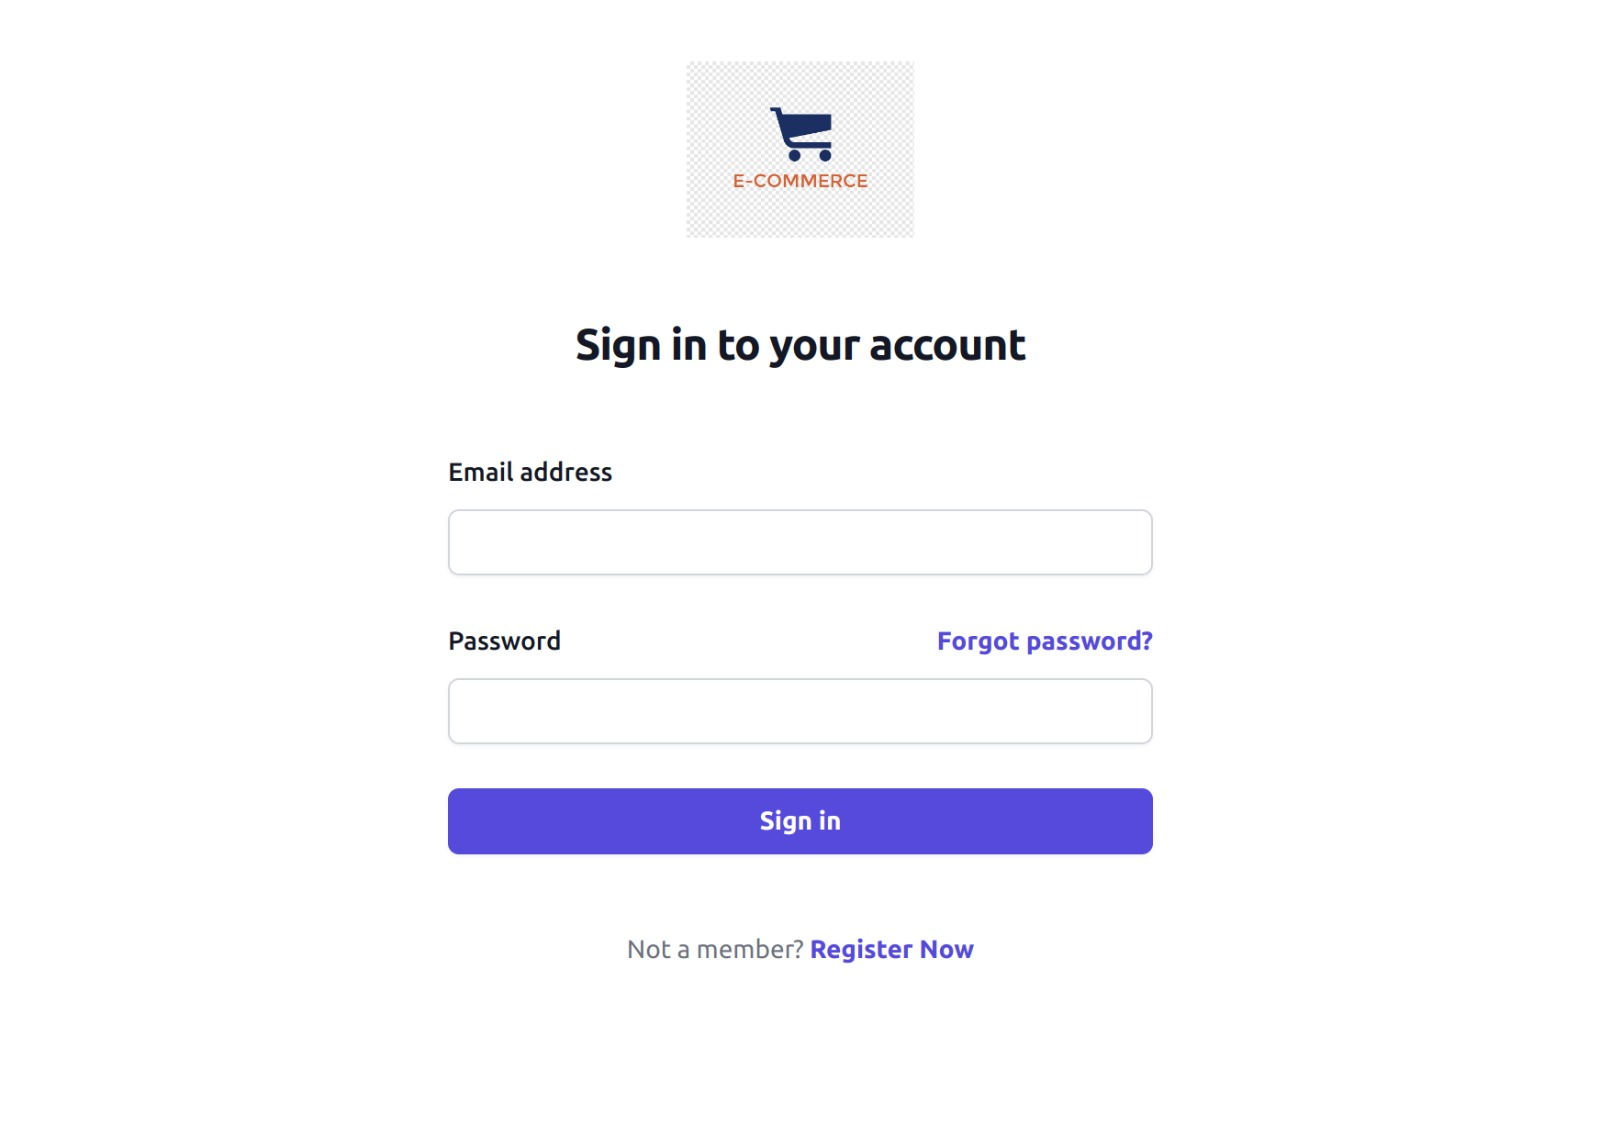
\includegraphics[width=0.8\textwidth]{sign_in.jpg} % Adjust width here
    \caption{Sign In Interface} % Add a caption
\end{figure}

\vspace{1cm} % Adjust vertical space

\begin{figure}[h!] % Use the figure environment
    \centering
    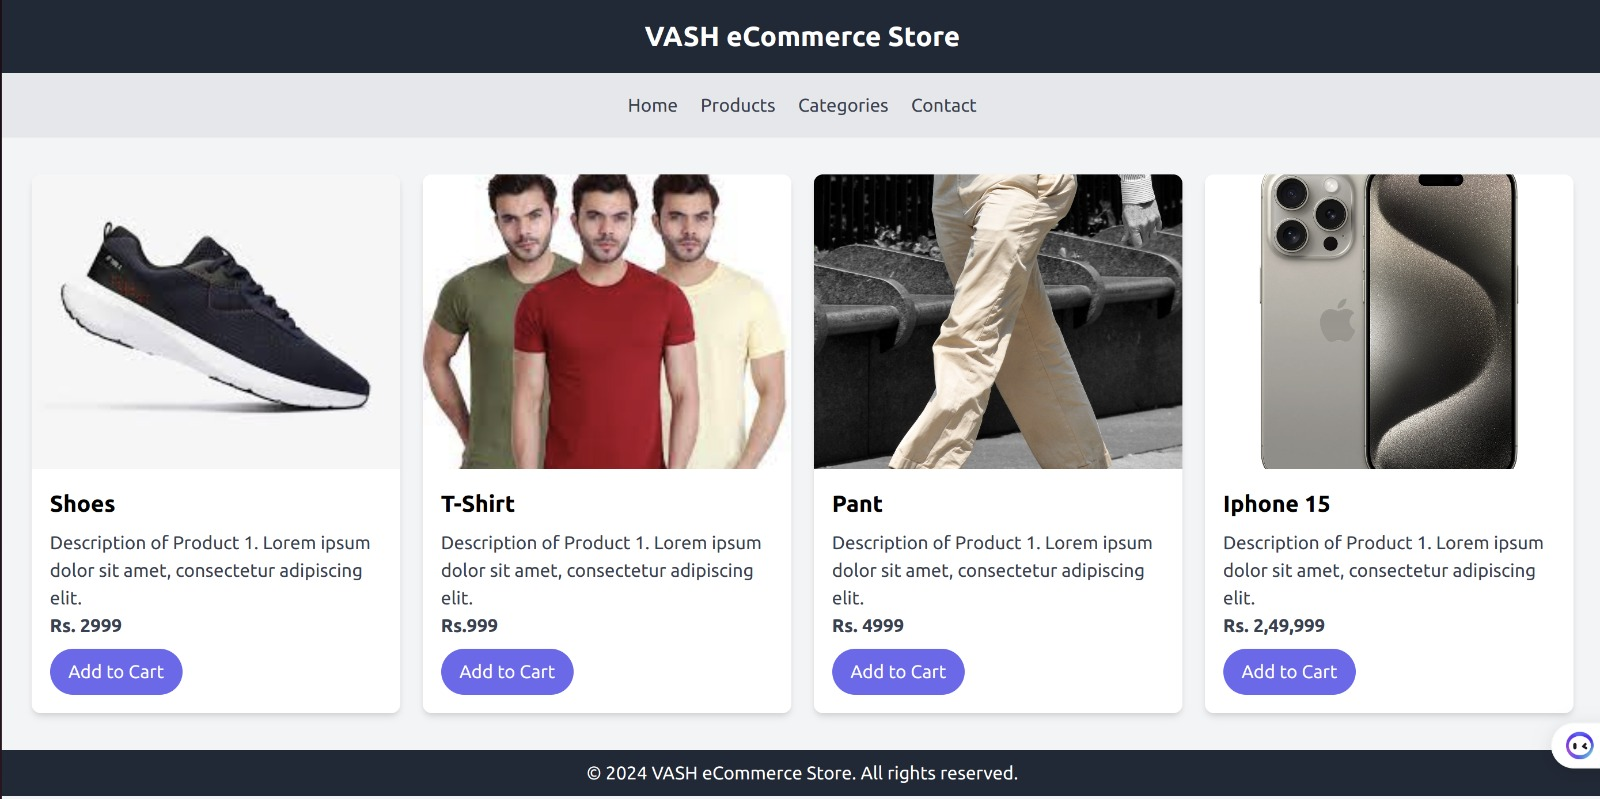
\includegraphics[width=0.8\textwidth]{dashboard.jpg} % Adjust width here
    \caption{Dashboard Interface} % Add a caption
\end{figure}

\vspace{1cm} % Adjust vertical space

\begin{figure}[h!] % Use the figure environment
    \centering
    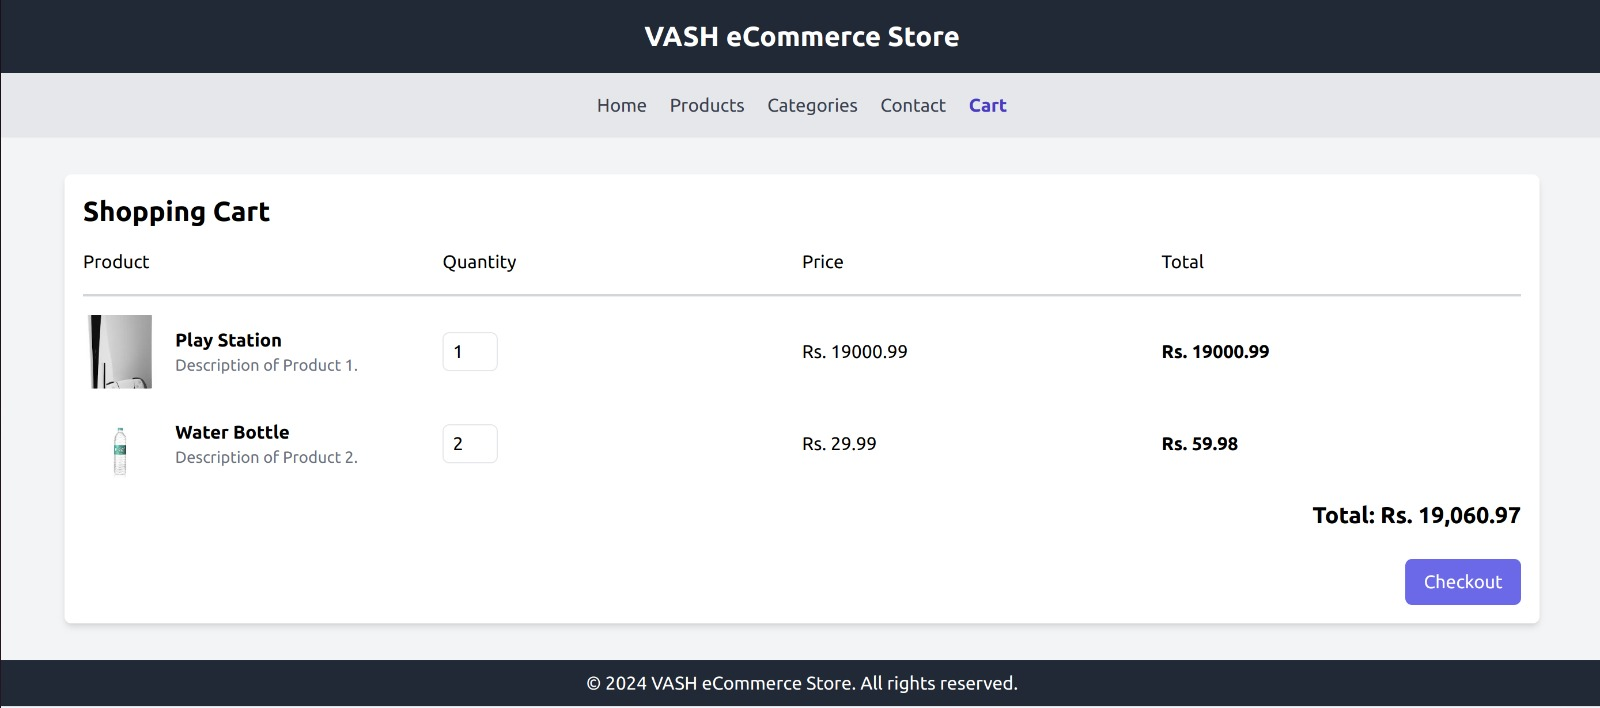
\includegraphics[width=0.8\textwidth]{cart.jpg} % Adjust width here
    \caption{Cart Interface} % Add a caption
\end{figure}

\vspace{1cm} % Adjust vertical space

\begin{figure}[h!] % Use the figure environment
    \centering
    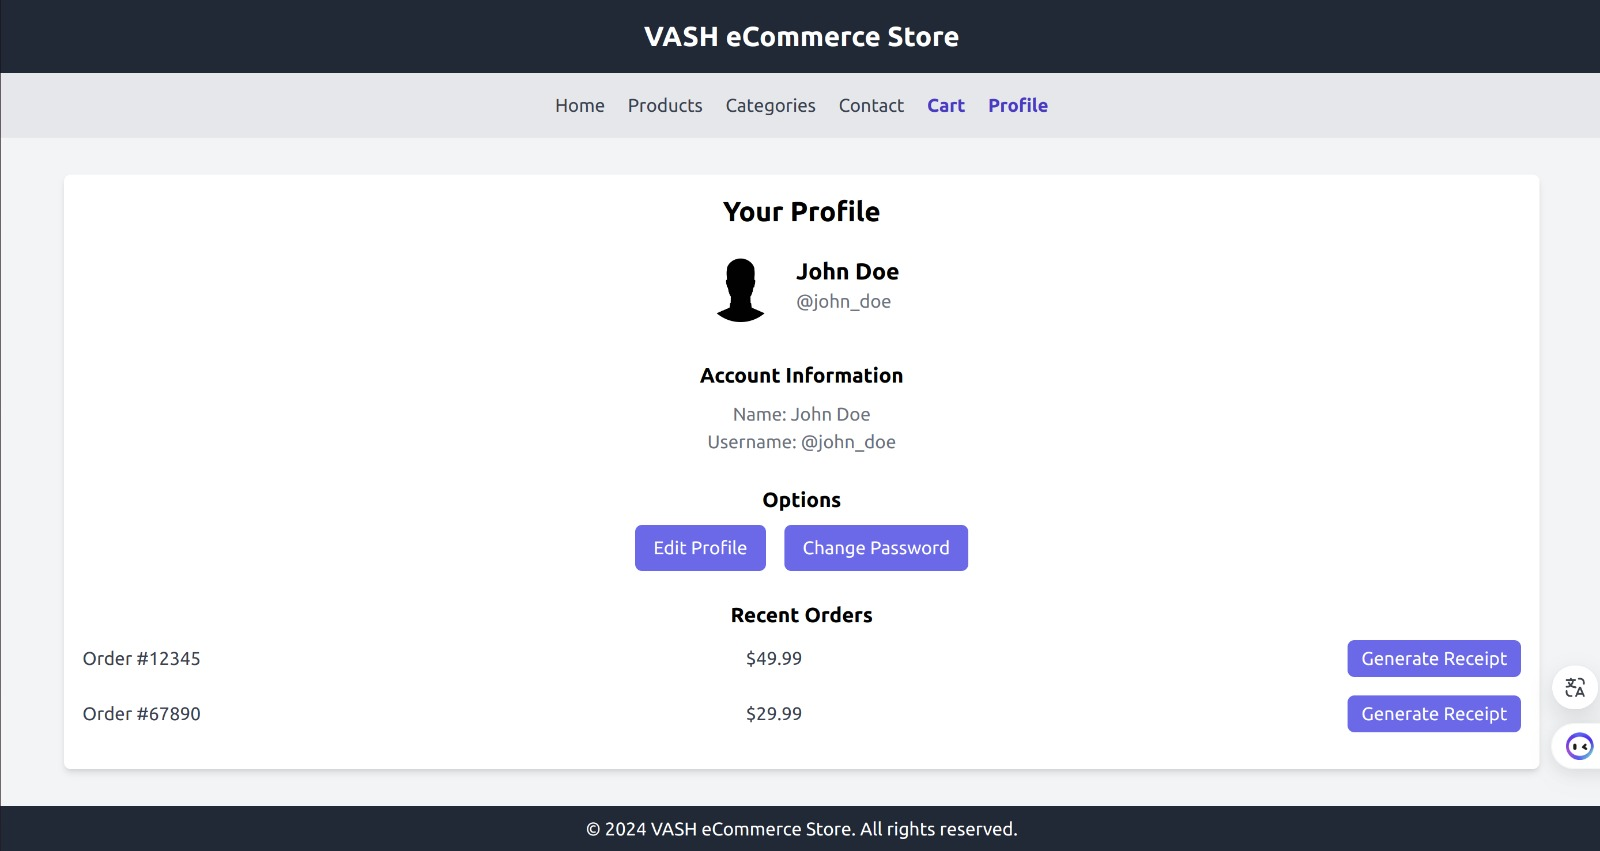
\includegraphics[width=0.8\textwidth]{profile.jpg} % Adjust width here
    \caption{Profile Interface} % Add a caption
\end{figure}
\newpage
\section{Future Extensions}
\begin{itemize}[label=-]
    \item Payment Gateway: Integration with a secure payment gateway for online transactions.
    \item Recommendation/View Similar Items: Implement a recommendation system based on user preferences and browsing history.
    \item Daily Revenue for Admin: Provide a feature for admins to track daily revenue and sales statistics.
\end{itemize}

\textbf{Note}: This SRS document provides an outline of the requirements for the development of the online platform. Detailed specifications, design, and implementation will be further elaborated during the development process.
\end{document}

